\documentclass[a4paper]{article}

% Includes packages relevant to Senior Lab

% character set specifications
\usepackage[english]{babel}
\usepackage[utf8]{inputenc}

% increased vertical spacing for tables
\newcommand\topVspace{\rule{0pt}{2.6ex}}      
\newcommand\bottomVspace{\rule[-1.2ex]{0pt}{0pt}} 

% extra unicode characters
\DeclareUnicodeCharacter{3BC}{\(\mu\)}
\DeclareUnicodeCharacter{3C1}{\(\rho\)}
\DeclareUnicodeCharacter{2080}{\(_0\)}
\DeclareUnicodeCharacter{2081}{\(_1\)}
\DeclareUnicodeCharacter{2082}{\(_2\)}
\DeclareUnicodeCharacter{3B5}{\(\epsilon\)}
\DeclareUnicodeCharacter{3B1}{\(\alpha\)}

% SI Units
\usepackage{siunitx}

% extra SI units
\DeclareSIUnit\gauss{G}

% enable scientific notation
\sisetup{scientific-notation = engineering, exponent-to-prefix}

% draw pretty lines
\usepackage{tikz}
\usetikzlibrary{datavisualization}
\usepackage{circuitikz}

% manual tabbing
\setlength{\parindent}{0pt}
\def\qq{\qquad}

% include graphics
\usepackage{graphicx}

% increased control over figure placement
\usepackage{float}

% box answers
\usepackage{tcolorbox}

% enable multiple section levels
\usepackage{titlesec}

% define `\subsubsubsection` command
\titleclass{\subsubsubsection}{straight}[\subsection]
\newcounter{subsubsubsection}[subsubsection]
\renewcommand\thesubsubsubsection{\thesubsubsection.\arabic{subsubsubsection}}
\titleformat{\subsubsubsection}
        {\normalfont\normalsize\bfseries}{\thesubsubsubsection}{1em}{}
\titlespacing*{\subsubsubsection}
{0pt}{3.25ex plus 1ex minus .2ex}{1.5ex plus .2ex}
\setcounter{secnumdepth}{4}

% get align environment (among other things)
\usepackage{amsmath}

% bold in math mode
\usepackage{bm}

% get \mathbb (among other things)
\usepackage{amssymb}

\usepackage{array}

% plotting
\usepackage{pgfplots}

% enable external references
\usepackage{hyperref}

% include code
\usepackage[cache=false]{minted}
\setminted{linenos, frame=lines, texcomments}

% adjust margins of individual pages (for shoving figures into place)
\usepackage{changepage}

% rotate figures
\usepackage{rotating}


\usepackage{subfigure}

\usepackage{caption}
\renewcommand{\thetable}{\arabic{section}.\arabic{table}}
\newcommand\T{\rule{0pt}{2.6ex}}       % Top strut
\newcommand\B{\rule[-1.2ex]{0pt}{0pt}} % Bottom strut

\begin{document}
\title{PHY 4210-01 Senior Lab \\Lab C1:  Mathematical Models of Chaotic Physical Systems }

\author{Sarah Arends \\
        Jacquelyne Miksanek \\
        Ryan Wojtyla \\ \\
        Instructor: Gus Azelis}

\date{\today}


\maketitle

\begin{abstract}
%physics of experiment
%apparatus used
%what was measured
%Results
\qq Chaotic behavior was studied by creating mathematical models and altering key parameters. A simple chaotic model was then observed by measuring time intervals of droplet formation from a leaking faucet. A small change in initial conditions can equate to much larger changes in the behavior of a system. The Feigenbaum number was calculated to be 5.

\end{abstract}

\newpage

\tableofcontents

\newpage

\section{The Logistic Equation}
\qq A population model can be represented with equation \ref{eq:log}, where $0<x_n<1$ and $r<4$. These parameters can be modified to observe the onset of chaotic behavior. The period doubling and chaotic regions will be investigated.

\begin{equation}
x_{n+1} = r x_n (1-x_n)
\label{eq:log}
\end{equation}

\subsection{Period Doubling Region of the Logistic Equation}
% progression of x_n for perioud doubling
\qq A period doubling region exists for $r<3.56994$. Plots of $x_n$ versus $x$ are produced for $0<r<3.56994$. Figure \ref{pdoub1} shows this behavior for a range of $r$ values. For $r<3$, the set of $x_n$ converge to a particular value, although they may fluctuate for the first few iterations. Around $r=3$ the values of $x_n$ oscillate between two values, as seen in figure \ref{pdoub1}. Around $r=3.5$, the values of $x_n$ begin oscillating between 4 values. This exhibits the period doubling region.

% xn vs n graph
\begin{figure}[H]
\centering
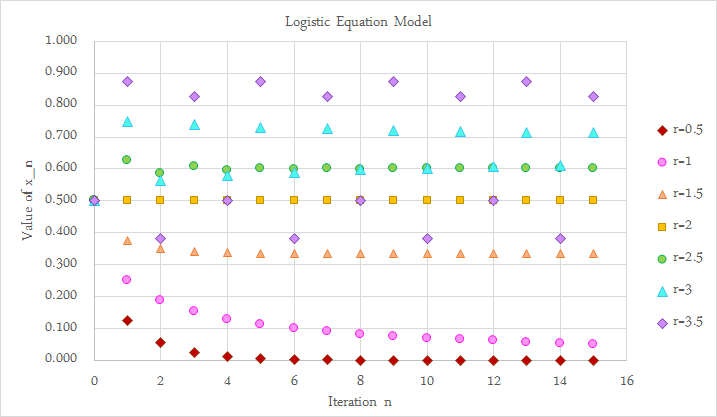
\includegraphics[width=1\textwidth]{pdoub.png}
\captionof{figure}{Series of $x_n$ vs $x$ for varying parameters $r<3.56994$. Plots of $x_n$ versus $x$ are produced for initial condition $x_0=0.5$. This is the period doubling region.}
\label{pdoub1}
\end{figure}

% feigenbaum
In the period doubling region, the period doubling parameters allows for a limit on the quantity $\frac{r_i - r_{i-1}}{r_{i+1} - r_i}$ equal to the Feigenbaum number, 4.66920. Here, $r_i$ is the value of $r$ during the $i^{th}$ period doubling. As mentioned previously, the data set will oscillate between two points for some r, then oscillate between four points for a greater r, and so on. Figure \ref{fein} shows the r values that correspond to oscillation between 2, 4, and 8 values. Their associated parameters will constitute $r_{i-1}$, $r_i$, and $r_{i+1}$, respectively.

\newpage

\begin{figure}[H]
\centering
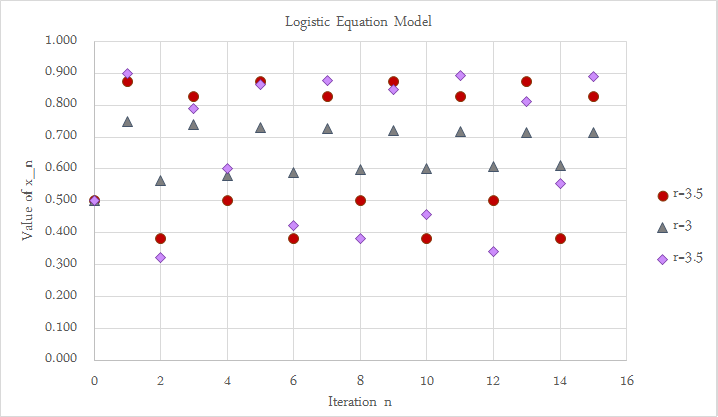
\includegraphics[width=1\textwidth]{fein.png}
\captionof{figure}{Series of $x_n$ vs $x$ for three r values, used to compute the Feigenbaum number.}
\label{fein}
\end{figure}

The experimental value for the Feigenbaum number is calculated as follows:
\begin{align*}
F
&= \frac{r_i - r_{i-1}}{r_{i+1} - r_i} \\
&= \frac{3.5-3}{3.6-3.5} \\
&= 5 \\
\end{align*}

This is roughly equal to the expected value of $F=4.6692$, with a percent error of $\delta F = 7.08 \%$. This error is a result of the approximation of the $r$ values that correspond to the start of each successive period doubling region, as there is no clear demarcation between these regions. Thus, there exists a random error in the determination of $r_{i-1}$, $r_i$, and $r_{i+1}$.

%n+1 vs n description
The period doubling region is further investigated by constructing a plot of $x_{n+1}$ versus $x_n$. For larger values of the parameter $r$, where periodicity begins emerging, ordered pairs $( x_n , x_{n+1} )$ began overlapping, as they repeat the same values in a given period. For smaller values of $r$, nearby $x_n$ values will also have nearby values for $x_{n+1}$. This trend is shown in figure \ref{pdoub1_n1vn}.

%n+1 vs n plot
\begin{figure}[H]
\centering
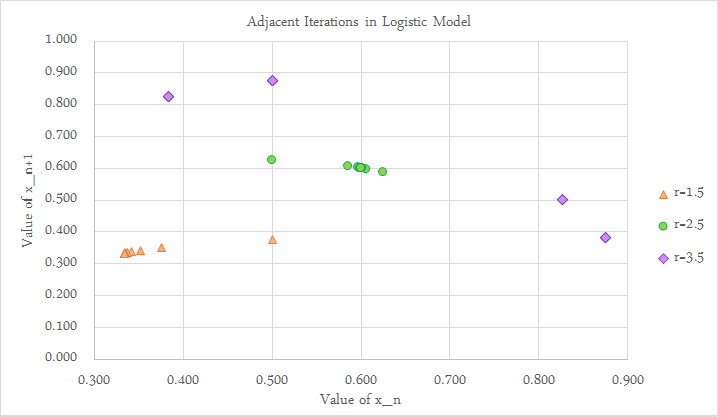
\includegraphics[width=1\textwidth]{pdoub_n1vn.png}
\captionof{figure}{The data from figure \ref{pdoub1} was re-processed for three $r$ values to show the relationship between $x_n$ values for adjacent iterations}
\label{pdoub1_n1vn}
\end{figure}

\subsection{Chaotic Region of the Logistic Equation}
% Part b and c
\qq A chaotic region occurs for $r>3.56994$. Plots of $x_n$ versus $x$ are produced for this region and graphed in figure \ref{chaos1}. The distributions for each $r$ value appear seemingly random because, although the system is deterministic, it is very sensitive to small changes.

% xn vs n graph, varying r
\begin{figure}[H]
\centering
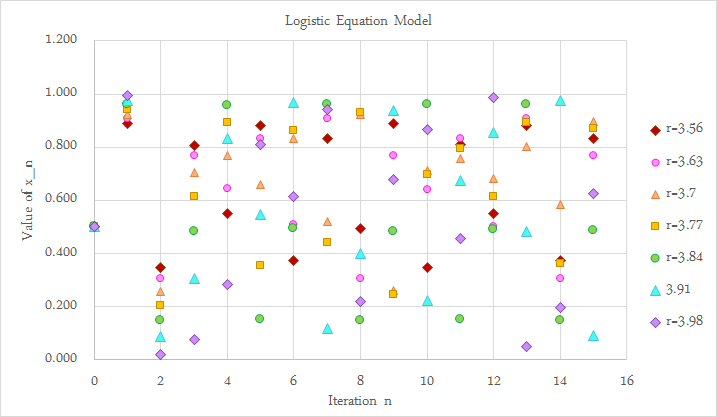
\includegraphics[width=1\textwidth]{chaos1.png}
\captionof{figure}{Series of $x_n$ vs $x$ for varying parameters $r>3.56994$. Plots of $x_n$ versus $x$ are produced for initial condition $x_0=0.5$. This is the chaotic region.}
\label{chaos1}
\end{figure}

\newpage 
% varying x_0
The behavior of $x_n$ is investigated by varying the initial condition $x_0$ by small amounts. A small change in this initial condition will produce even greater variations as $n$ gets large. For the range of $n$ values shown in figure \ref{varyx0}, the percent change in $x_n$ values was computed between the series corresponding to initial conditions $x_0=0.8$ and $x_0=0.801$. The percent change was minimized for the zeroth iteration, at $0.125\%$. The difference was at a maximum of $437\%$ for the fourteenth iteration, and the change was closest to $1\%$ for the eighth iteration.

% xn vs n graph, varying x0
\begin{figure}[H]
\centering
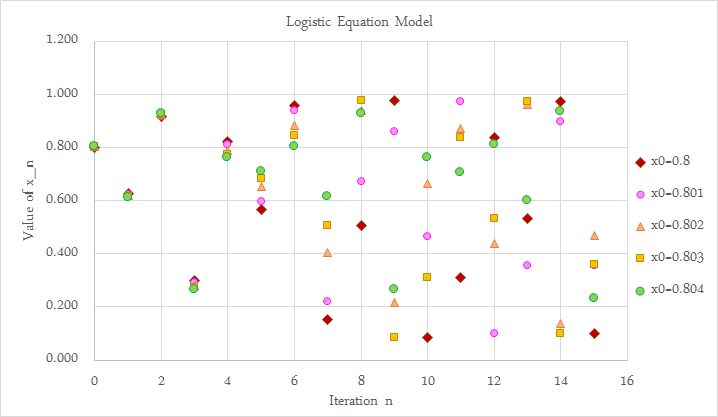
\includegraphics[width=1\textwidth]{varyx0.png}
\captionof{figure}{Series of $x_n$ vs $x$ for varying initial conditions $x_0$. Plots of $x_n$ versus $x$ are produced for $r=3.91$, which falls in the chaotic region.}
\label{varyx0}
\end{figure}

%n+1 vs n description
The chaotic region is further investigated by constructing a plot of $x_{n+1}$ versus $x_n$. An interesting pattern emerges, as shown in figure \ref{chaos_n1vn}, that depicts how a chaotic process is still deterministic. For all three $r$ values, the relationship between $x_{n+1}$ and $x_n$ follows the same roughly quadratic distribution. Thus, there is a relatively predictable relationship between $x_n$ and $x_{n+1}$. For a small neighborhood of variation around $x_n$, we can also define a small neighborhood of variation around the corresponding values of $x_{n+1}$.

%n+1 vs n plot
\begin{figure}[H]
\centering
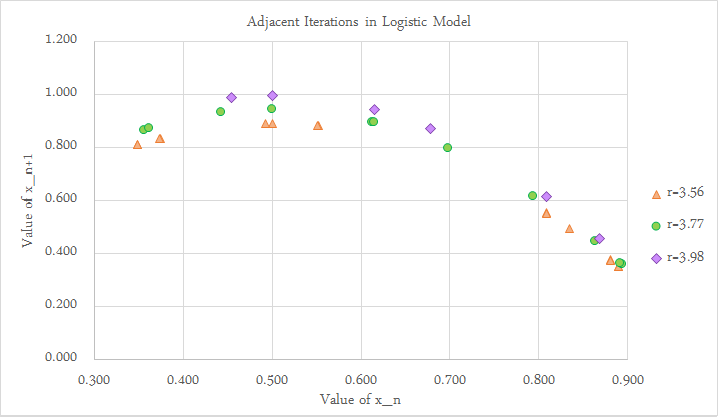
\includegraphics[width=1\textwidth]{chaos_n1vn.png}
\captionof{figure}{The data from figure \ref{chaos1} was re-processed for three $r$ values to show the relationship between $x_n$ values for adjacent iterations}
\label{chaos_n1vn}
\end{figure}

\section{Lyapunov Experiments}
% Part d and e

\qq The function provided for determining Lyapunov exponents

\begin{equation*}
  \lambda = \lim\limits_{x \rightarrow \infty} \frac{1}{n} \sum^n_{k=0} 
  \ln \left( \left| \frac{d f(x_k)}{dx} \right| \right)
\end{equation*}

has been implemented in Julia; the source code is shown in Section
\ref{cod:lyapunov}. In the regular region, \( r < 3.56994 \), while in the
chaotic region, \( r \geq 3.56994 \). While the inflection point of \( r \) has
been shown to be closer to \( r = 3 \), it is clearly seen that \( \lambda < 0
\) in the regular region and \( \lambda > 0 \) in the chaotic region.

\qq To calculate \( \lambda \) for \( x_0 = 0.7 \), \( r = 2.5 \), and \( n = 20
\), the argument array {\tt lyaARGS = [0.7, 2.5, 20]} is constructed and used by
the program. Since \( r \) is well within the regular region, a call to the
function that calculates the Lyapunov exponent, {\tt lya(iters, x -> logFunc(r,x),
  initCond, r)}, produces a negative value, \( \lambda = -0.853 \). Similarly,
for \( r = 3.7 \), \( \lambda = 0.420 \), a positive value indicative of this
larger \( r \)'s chaotic nature. 

\section{Visualization of Chaos}

\qq The difference between the regular and chaotic regions can be clearly seen
by plotting the logistic function \( f(x_n) = x_{n+1} = r x_n (1 - x_n) \) for different
values of \( r \). Such a plot is shown in Figure \ref{gph:xnVr}. While the
inflection point displayed in the graph is less than the theoretical \( r =
3.56994 \), a dramatic distinction between the two regions can nonetheless be
clearly seen.

\begin{figure}[H]
  \begin{center}
    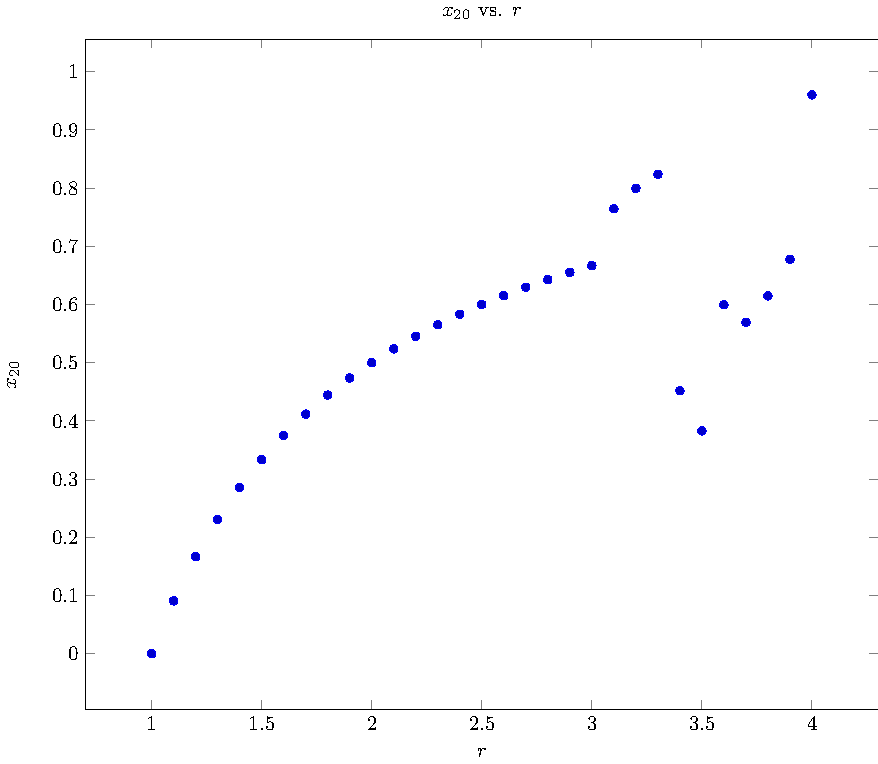
\includegraphics[width=1.0\textwidth]{Plots/PartE/xnVr.pdf}
  \end{center}
  \caption{The plot of \( x_n \) for several values of \( r \), where \( x_0 =
    0.7 \) and \( n = 20 \). The Julia program seen in Section \ref{cod:xnVr}
    was called with the command line arguments {\tt 0.7 20} to generate the
    values.}
  \label{gph:xnVr}
\end{figure}

\section{Water Drop Experiment}

\qq To collect chaotic data, the frequency with which drops formed at a sink was
recorded for a specified number of total drops. Six trials were conducted, and the
results are plotted below. Although the results were meant to be chaotic,
some of the trials show drops being produced at a fairly regular rate. The
trials in Figures \ref{fig:test3} and \ref{fig:test4} produced more regular
results than the other trials; the data points exhibit less variety than in the
other plots, which, although they are less than totally chaotic, scatter fairly
widely. 

% plots 1 and 2
\begin{figure}[H]
\centering
\begin{minipage}{.5\textwidth}
  \centering
  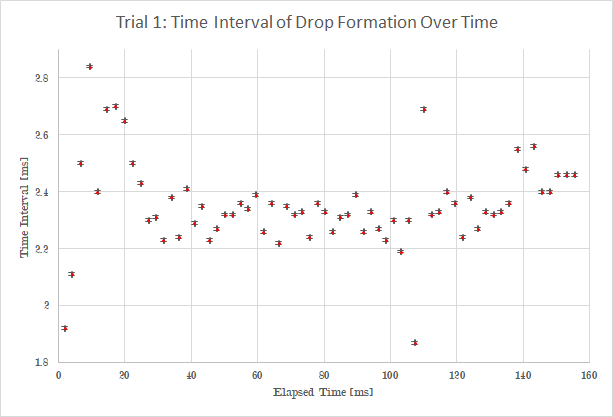
\includegraphics[width=\linewidth]{sink1.png}
  \captionof{figure}{Trial 1}
  \label{fig:test1}
\end{minipage}%
\begin{minipage}{.5\textwidth}
  \centering
  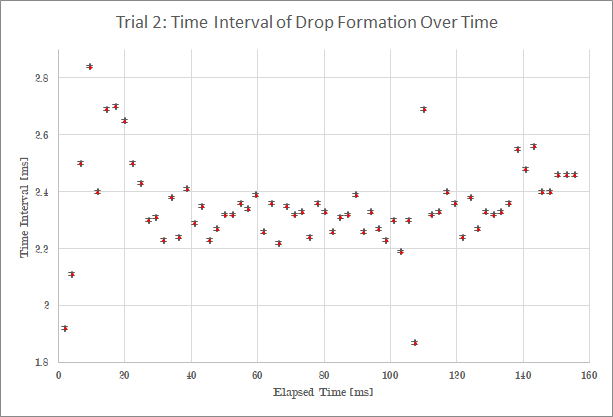
\includegraphics[width=\linewidth]{sink2.png}
  \captionof{figure}{Trial 2}
  \label{fig:test2}
\end{minipage}
\end{figure}

% plots 3 and 4
\begin{figure}[H]
\centering
\begin{minipage}{.5\textwidth}
  \centering
  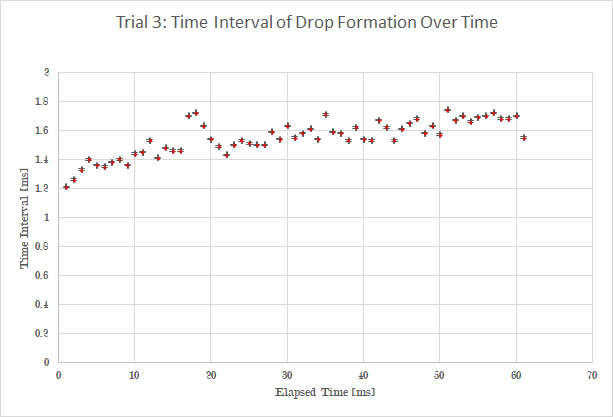
\includegraphics[width=\linewidth]{sink3.png}
  \captionof{figure}{Trial 3}
  \label{fig:test3}
\end{minipage}%
\begin{minipage}{.5\textwidth}
  \centering
  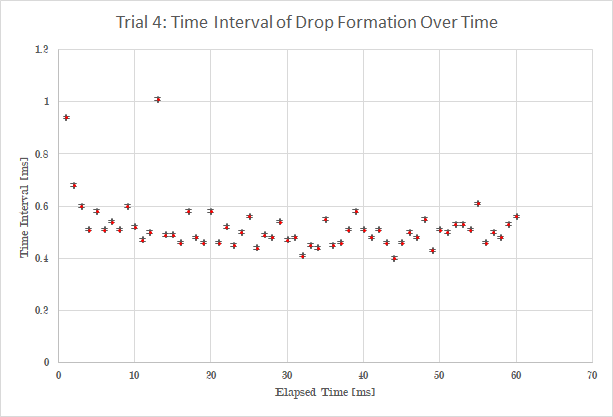
\includegraphics[width=\linewidth]{sink4.png}
  \captionof{figure}{Trial 4}
  \label{fig:test4}
\end{minipage}
\end{figure}

% plots 5 and 6
\begin{figure}[H]
\centering
\begin{minipage}{.5\textwidth}
  \centering
  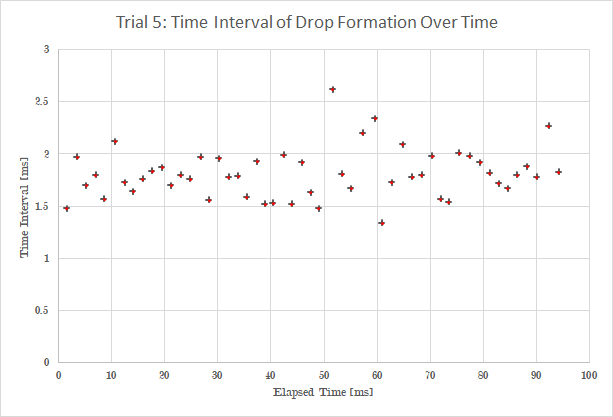
\includegraphics[width=\linewidth]{sink5.png}
  \captionof{figure}{Trial 5}
  \label{fig:test5}
\end{minipage}%
\begin{minipage}{.5\textwidth}
  \centering
  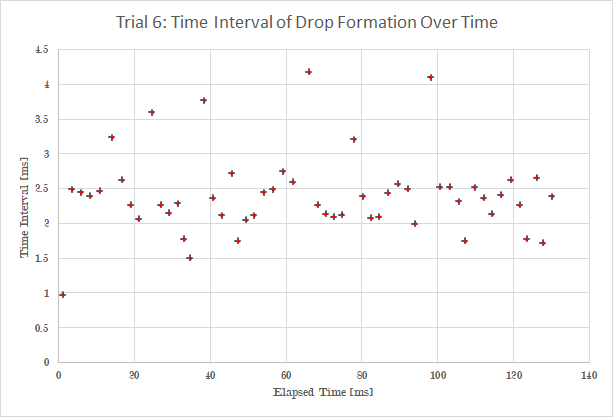
\includegraphics[width=\linewidth]{sink6.png}
  \captionof{figure}{Trial 6}
  \label{fig:test6}
\end{minipage}
\end{figure}

\section{Sources of Error}

\qq The only source of error in the experiment is present in the times at which
the water drops formed at the sink. This is random error in measurement because
it is dependent upon the reaction time of the observer. It has the nominal
effect of introducing slightly more chaos than there otherwise would have been. 

\section{Conclusion}
%Brief summary, discussion of results and theory
\qq Graphical analysis was used to understand the behavior of the logistic model in both the period doubling and chaotic regimes. The Feigenbaum number was successfully computed with 7 percent error. The lyapunov exponent was shown to be negative in the regular region and positive in the chaotic region, with some error in the inflection point. A dripping faucet experiment showed the chaotic behavior that was previously modeled.

\section{Appendices}

\subsection{Appendix A: Source Code}

\subsubsection{Lyapunov Exponent Calculation}
\label{cod:lyapunov}
%Lyapunov.jl

\subsubsection{\( x_n \) Calculations for Different \( r \)s}
\label{cod:xnVr}
%xnVr.jl

\end{document}
